\chapter{Training Transformers at Scale}

\section*{Why This Matters}

Training transformer models represents the most significant technical and financial investment in AI system development. Understanding training infrastructure requirements, distributed training strategies, and optimization techniques is essential for accurate project planning, vendor evaluation, and infrastructure investment decisions.

The scale of transformer training has increased dramatically. GPT-2 required approximately 1,000 GPU-days; GPT-3 required 3,000-5,000 GPU-days; recent large models require tens of thousands of GPU-days. These training runs cost hundreds of thousands to millions of dollars, making training efficiency and reliability critical business concerns.

This chapter examines the technical architecture of transformer training at scale, focusing on distributed training strategies, memory optimization techniques, and the engineering trade-offs that determine training costs and timelines.

\section{Training Pipeline Architecture}

\subsection{End-to-End Training Flow}

Transformer training involves multiple coordinated stages, each with specific resource requirements and failure modes. The complete pipeline includes data loading, forward computation, backward computation, gradient aggregation, parameter updates, and checkpointing.

\textbf{Data Loading and Preprocessing}: Training data flows from storage through preprocessing pipelines to GPU memory. For large-scale training, data loading often becomes a bottleneck. A single A100 GPU can process data faster than typical storage systems can supply it, necessitating parallel data loading, prefetching, and in-memory caching.

\textbf{Forward and Backward Passes}: The model processes batches through forward computation (generating predictions) and backward computation (computing gradients). For BERT-base, a single forward-backward pass on 32 sequences requires approximately 0.6 seconds on A100 hardware. Scaling to larger models or batches increases this proportionally.

\textbf{Gradient Aggregation}: In distributed training, gradients computed across multiple GPUs must be aggregated before parameter updates. This communication step can consume 20-40\% of total training time if not optimized properly.

\textbf{Parameter Updates and Checkpointing}: After gradient aggregation, optimizers update parameters. Periodically (every 1,000-10,000 steps), the training state is checkpointed to persistent storage, enabling recovery from hardware failures.

\begin{figure}[htbp]
\centering
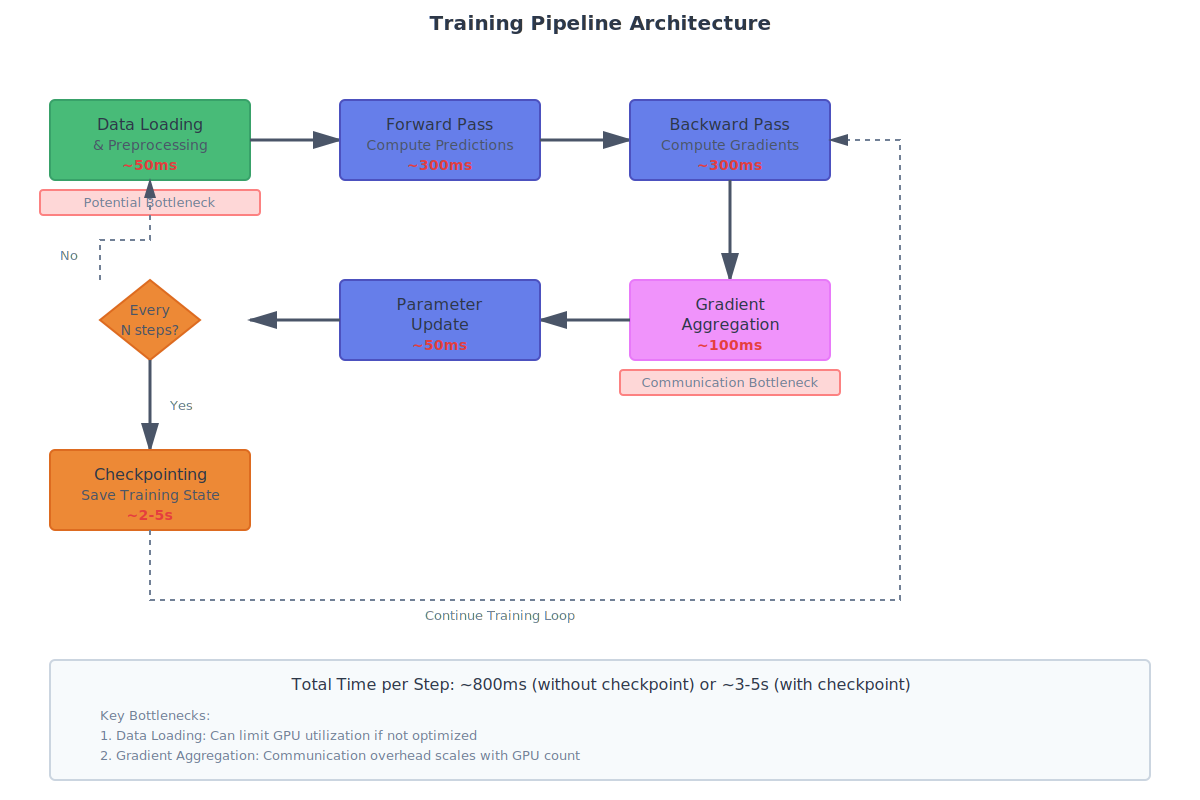
\includegraphics[width=0.95\textwidth]{chapters/diagrams/chapter04_training_pipeline_a1b2c3d4.pdf}
\caption{Complete training pipeline showing data flow, computation stages, and communication patterns. Data loading and gradient aggregation represent primary bottlenecks in distributed training.}
\label{fig:training_pipeline}
\end{figure}

\subsection{Training Time Estimation}

Training time can be estimated from model size, dataset size, and hardware specifications:

\begin{center}
\fbox{\parbox{0.85\textwidth}{
\centering
Training Time = (Parameters $\times$ Tokens $\times$ 6) / (GPU FLOPS $\times$ Utilization $\times$ GPU Count)
}}
\end{center}

The factor of 6 accounts for forward pass (1×), backward pass (2×), and additional overhead (3×). Utilization typically ranges from 30-50\% of theoretical peak performance.

For GPT-2 (1.5B parameters, 40B tokens, 8× V100 GPUs):
\begin{itemize}
    \item Computation: 1.5B $\times$ 40B $\times$ 6 = 360 $\times$ 10$^{18}$ operations
    \item GPU capacity: 8 GPUs $\times$ 125 TFLOPS $\times$ 0.4 utilization = 400 TFLOPS effective
    \item Training time: 360 $\times$ 10$^{18}$ / 400 $\times$ 10$^{12}$ = 900,000 seconds $\approx$ 250 hours $\approx$ 10 days
\end{itemize}

This matches reported GPT-2 training times, validating the estimation approach.


\section{Distributed Training Strategies}

\subsection{Data Parallelism}

Data parallelism replicates the model across multiple GPUs, with each GPU processing different data batches. This approach scales efficiently for models that fit in single-GPU memory.

\textbf{Implementation}: Each GPU maintains a complete model copy. During training, each GPU processes its batch independently, computes gradients, then all GPUs synchronize gradients through all-reduce operations. After synchronization, each GPU applies identical parameter updates.

\textbf{Scaling Characteristics}: Data parallelism scales nearly linearly up to 64-128 GPUs for large models. Beyond this point, communication overhead dominates, reducing efficiency. For BERT-base with optimized communication (NCCL 2.20+), 8-way data parallelism achieves 7.5-7.8× speedup (94-97\% efficiency); 64-way achieves 55-58× speedup (86-91\% efficiency). Older configurations achieve 75-80\% efficiency at 64-way scale.

\textbf{Memory Requirements}: Each GPU requires full model memory (parameters, gradients, optimizer states). For models exceeding single-GPU memory, data parallelism alone is insufficient.

\subsection{Model Parallelism}

Model parallelism partitions the model across multiple GPUs, enabling training of models too large for single-GPU memory. Two primary approaches exist: pipeline parallelism and tensor parallelism.

\textbf{Pipeline Parallelism}: Divides the model by layers. GPU 1 processes layers 1-4, GPU 2 processes layers 5-8, etc. Data flows through GPUs sequentially. This approach introduces pipeline bubbles—periods where GPUs idle waiting for data—reducing efficiency to 60-80\% typically.

\textbf{Tensor Parallelism}: Partitions individual layers across GPUs. A single matrix multiplication splits across multiple GPUs, which compute partial results and communicate to produce final outputs. This approach requires high-bandwidth interconnects (NVLink, InfiniBand) and achieves 80-90\% efficiency with proper implementation.

\textbf{Hybrid Approaches}: Production systems typically combine data parallelism, pipeline parallelism, and tensor parallelism. GPT-3 training used 8-way tensor parallelism, 16-way pipeline parallelism, and 8-way data parallelism, totaling 1,024 GPUs.

\begin{tcolorbox}[colback=purple!5!white,colframe=purple!75!black,title=\textbf{MENTAL MODEL: Distributed Training Decision Tree}]

\textbf{Principle:} Choose parallelism strategy based on model size and available hardware, not theoretical performance.

\textbf{Decision Framework:}

\textbf{If model fits in single GPU (less than 40GB):}
\begin{itemize}
    \item Use data parallelism only
    \item Scale to 8-64 GPUs for 7-55× speedup
    \item Efficiency: 90-95\% (minimal communication overhead)
\end{itemize}

\textbf{If model fits in single GPU but training is slow:}
\begin{itemize}
    \item Add data parallelism (2-8 GPUs)
    \item Cost: 2-8× hardware, gain: 1.9-7.5× speedup
    \item Break-even: If training takes more than 2 days, parallelism pays off
\end{itemize}

\textbf{If model exceeds single GPU (40-320GB):}
\begin{itemize}
    \item Use tensor parallelism (2-8 GPUs per model copy)
    \item Then add data parallelism across model copies
    \item Efficiency: 80-90\% (higher communication overhead)
\end{itemize}

\textbf{If model exceeds 8-GPU capacity (greater than 320GB):}
\begin{itemize}
    \item Add pipeline parallelism (layers across GPUs)
    \item Efficiency drops to 60-80\% (pipeline bubbles)
    \item Only use when necessary—complexity is high
\end{itemize}

\textbf{Example:} BERT-base (440MB parameters, 6GB training memory). Fits in single A100 (80GB). Use data parallelism with 8 GPUs for 7.5× speedup. Training time: 10 days becomes 1.3 days. Cost: 8× hardware but 7.5× faster equals 1.07× total cost for 7.5× faster delivery.

\textbf{Red Flag:} "We'll use pipeline parallelism for faster training"—pipeline parallelism is for models that don't fit, not for speed. It's slower than data parallelism due to pipeline bubbles (60-80\% efficiency versus 90-95\%).

\end{tcolorbox}

\begin{figure}[htbp]
\centering
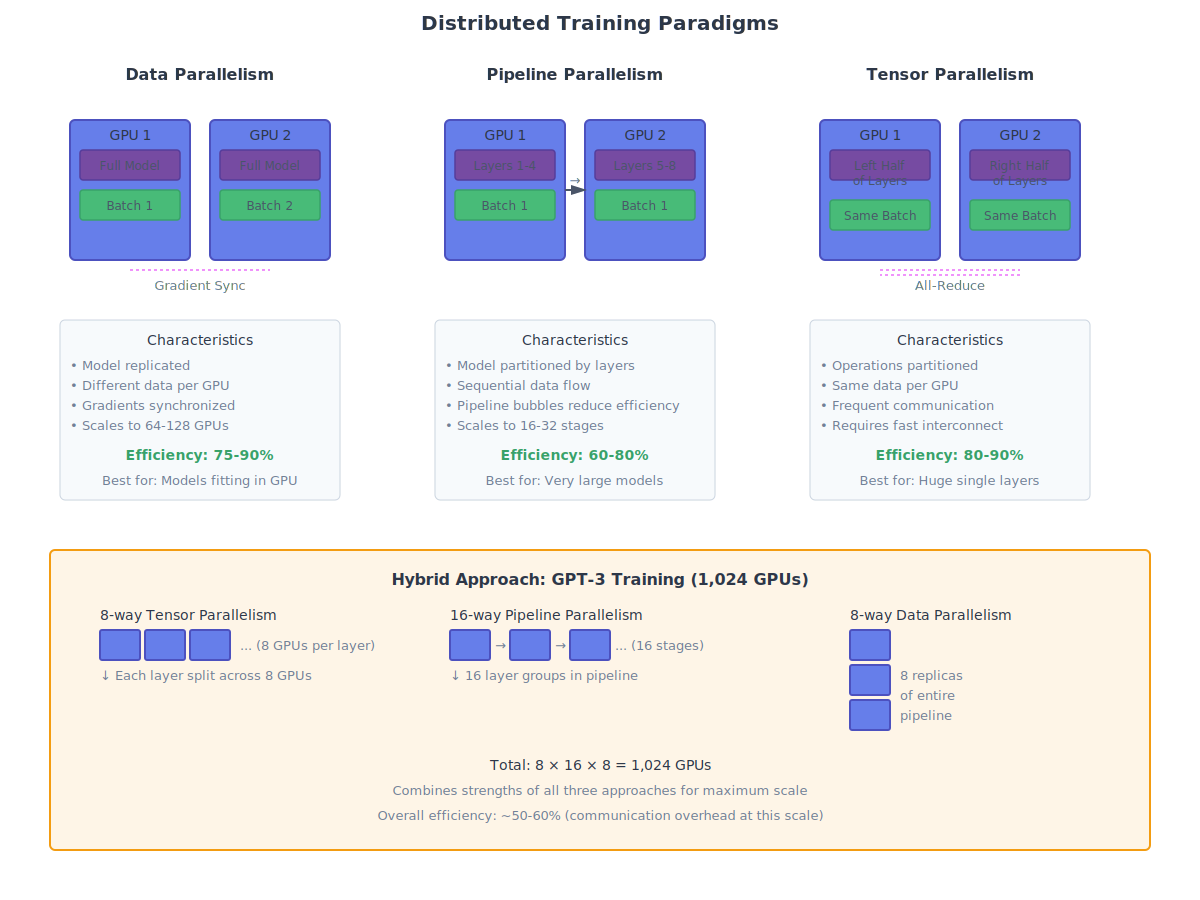
\includegraphics[width=0.9\textwidth]{chapters/diagrams/chapter04_distributed_training_e5f6g7h8.pdf}
\caption{Distributed training paradigms: data parallelism (model replication), pipeline parallelism (layer partitioning), and tensor parallelism (operation partitioning). Each approach presents different scaling characteristics and efficiency trade-offs.}
\label{fig:distributed_training}
\end{figure}

\subsection{Communication Optimization}

Distributed training efficiency depends critically on communication optimization. Gradient synchronization requires transferring gigabytes of data between GPUs, potentially consuming more time than computation.

\textbf{Gradient Accumulation}: Accumulates gradients over multiple micro-batches before synchronization, reducing communication frequency. This technique enables larger effective batch sizes without proportional memory increases.

\textbf{Mixed Precision Communication}: Communicates gradients in 16-bit precision while maintaining 32-bit precision for parameters. This halves communication volume with minimal accuracy impact.

\textbf{Gradient Compression}: Applies compression algorithms to gradients before communication. Techniques like gradient sparsification (transmitting only large gradients) can reduce communication by 100-1000× with careful tuning, though implementation complexity increases significantly.


\section{Memory Optimization Techniques}

\subsection{Activation Checkpointing}

Activation checkpointing (also called gradient checkpointing) trades computation for memory by recomputing activations during backward pass rather than storing them.

\textbf{Memory Savings}: Reduces activation memory from O(n $\times$ L) to O($\sqrt{n \times L}$), where n is batch size and L is layer count. For BERT-base, this reduces activation memory from 3.5 GB to approximately 1 GB—a 3.5× reduction.

\textbf{Computational Cost}: Increases training time by 20-33\% due to recomputation. The trade-off is favorable when memory constraints prevent training otherwise, or when larger batch sizes enabled by memory savings improve convergence sufficiently to offset recomputation costs.

\textbf{Selective Checkpointing}: Rather than checkpointing all layers, selective strategies checkpoint only expensive layers (attention layers) while storing cheap layer activations (normalization, residual connections). This approach achieves 2-2.5× memory reduction with only 10-15\% time increase.

\subsection{Mixed Precision Training}

Mixed precision training uses 16-bit floating-point (FP16) for most operations while maintaining 32-bit (FP32) precision where numerical stability requires it.

\textbf{Memory Benefits}: FP16 parameters and activations require half the memory of FP32, enabling 2× larger models or batch sizes on given hardware.

\textbf{Computational Benefits}: Modern GPUs (V100, A100, H100) include specialized FP16 hardware providing 2-8× throughput compared to FP32. For transformer training, mixed precision typically provides 1.5-2× speedup.

\textbf{Implementation Requirements}: Maintains master weights in FP32, performs forward and backward passes in FP16, then updates FP32 master weights. Loss scaling prevents gradient underflow in FP16 range. Modern frameworks (PyTorch, TensorFlow) provide automatic mixed precision, simplifying implementation.

\begin{figure}[htbp]
\centering
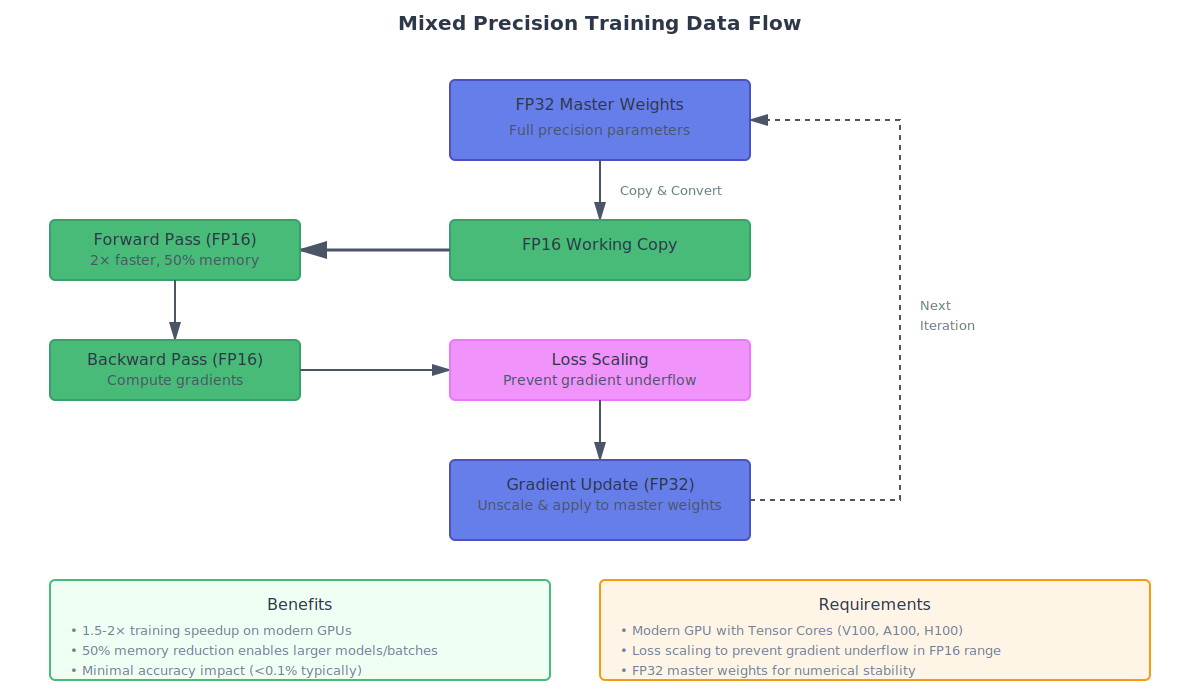
\includegraphics[width=0.9\textwidth]{chapters/diagrams/chapter04_mixed_precision_i9j0k1l2.pdf}
\caption{Mixed precision training data flow. Forward and backward passes use FP16 for speed and memory efficiency, while master weights remain in FP32 for numerical stability. Loss scaling prevents gradient underflow.}
\label{fig:mixed_precision}
\end{figure}

\subsection{Optimizer State Management}

Optimizer states (momentum, variance for Adam) consume significant memory—2× parameter memory for Adam. Several techniques reduce this overhead:

\textbf{Optimizer State Sharding}: Distributes optimizer states across GPUs rather than replicating them. Each GPU maintains optimizer states for a parameter subset, reducing per-GPU memory by GPU count. This technique, used in ZeRO optimizer, enables training models 4-8× larger on given hardware.

\textbf{8-bit Optimizers}: Quantizes optimizer states to 8-bit integers, reducing memory by 4× with minimal accuracy impact. Combined with state sharding, this enables training models 16-32× larger than naive implementations.

\textbf{CPU Offloading}: Stores optimizer states in CPU memory, transferring to GPU only during parameter updates. This trades memory for bandwidth, feasible when high-speed CPU-GPU interconnects (NVLink, PCIe 4.0) are available.


\section{Learning Rate Schedules}

\subsection{Warmup and Decay Strategies}

Learning rate schedules significantly impact training efficiency and final model quality. Transformer training typically employs warmup followed by decay.

\textbf{Linear Warmup}: Increases learning rate linearly from near-zero to target value over initial training steps. Typical warmup duration: 1-10\% of total training. This addresses optimizer initialization issues and prevents early training instability.

\textbf{Cosine Decay}: After warmup, learning rate follows cosine curve from peak to near-zero. This schedule enables aggressive exploration early and fine-tuning late, typically improving final performance by 1-3\% compared to constant learning rates.

\textbf{Inverse Square Root Decay}: Learning rate decays proportionally to $1/\sqrt{step}$. This schedule, used in original Transformer paper, provides gentler decay than cosine, sometimes preferred for very long training runs.

\begin{figure}[htbp]
\centering
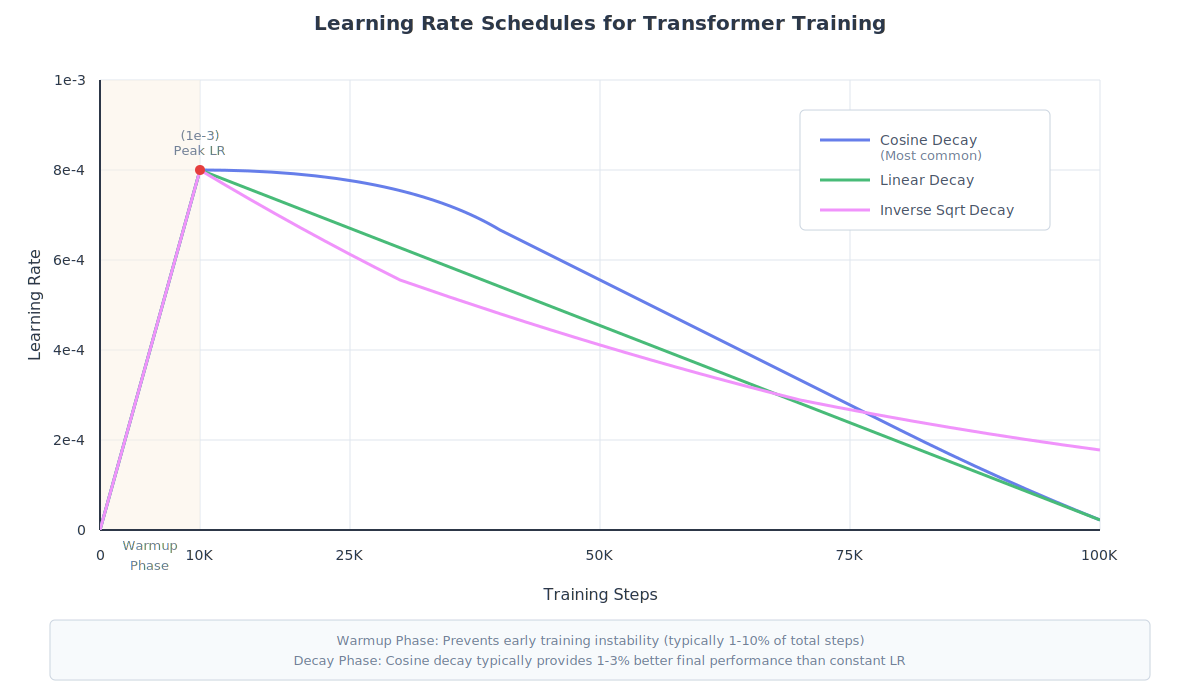
\includegraphics[width=0.9\textwidth]{chapters/diagrams/chapter04_learning_schedules_m3n4o5p6.pdf}
\caption{Common learning rate schedules for transformer training. Warmup prevents early instability; decay strategies balance exploration and convergence. Cosine decay typically provides best final performance.}
\label{fig:learning_schedules}
\end{figure}

\subsection{Adaptive Learning Rates}

Beyond scheduled decay, several techniques adapt learning rates based on training dynamics:

\textbf{Layer-wise Learning Rates}: Applies different learning rates to different layers. Early layers (closer to input) often benefit from smaller learning rates than later layers. This technique can improve convergence speed by 10-20\%.

\textbf{Gradient Clipping}: Limits gradient magnitude to prevent instability. Essential for transformer training, as attention mechanisms can produce large gradients. Typical clip values: 1.0-5.0 for gradient norm.

\textbf{Learning Rate Rewinding}: If training becomes unstable (loss spikes), rewinds to earlier checkpoint and reduces learning rate. This technique enables more aggressive initial learning rates while maintaining stability.


\section{Checkpointing and Fault Tolerance}

\subsection{Checkpoint Strategy}

Large-scale training runs span days or weeks, during which hardware failures are inevitable. Robust checkpointing is essential for training reliability.

\textbf{Checkpoint Frequency}: Balance between recovery time and checkpoint overhead. Typical strategy: checkpoint every 1,000-10,000 steps (1-4 hours of training). More frequent checkpointing reduces recovery time but increases storage I/O overhead.

\textbf{Checkpoint Content}: Full checkpoints include model parameters, optimizer states, learning rate schedule state, random number generator states, and data loader position. For BERT-base, full checkpoint size: approximately 2 GB. For GPT-3 scale: 350+ GB.

\textbf{Checkpoint Storage}: Checkpoints should be written to reliable distributed storage (not local GPU storage). Asynchronous checkpointing—writing checkpoints while training continues—prevents training interruption. This requires double-buffering checkpoint memory.

\subsection{Failure Recovery}

Hardware failures occur regularly in large-scale training. A 1,000-GPU training run experiences GPU failures approximately every 1-2 days on average.

\textbf{Automatic Recovery}: Production training systems detect failures and automatically restart from latest checkpoint. This requires orchestration systems (Kubernetes, Slurm) configured for automatic job restart.

\textbf{Partial Failure Handling}: In distributed training, single GPU failure can crash entire job. Elastic training—dynamically adjusting GPU count after failures—enables continued training with reduced resources until failed hardware is replaced.

\textbf{Checkpoint Validation}: Corrupted checkpoints can waste hours of training. Validation checks (parameter statistics, gradient norms) detect corruption before resuming training.


\section{Training Efficiency Optimization}

\subsection{Batch Size Optimization}

Batch size significantly impacts training efficiency, convergence speed, and final model quality.

\textbf{Large Batch Training}: Larger batches improve GPU utilization and reduce training time. However, very large batches can degrade final model quality. The critical batch size—beyond which larger batches don't improve convergence—varies by model and task but typically ranges from 256-2048 for transformers.

\textbf{Gradient Accumulation}: Simulates large batches without memory increase by accumulating gradients over multiple small batches before parameter updates. This enables effective batch sizes exceeding GPU memory limits.

\textbf{Batch Size Scaling}: When increasing batch size, learning rate should typically scale proportionally (linear scaling rule). Doubling batch size requires doubling learning rate to maintain convergence speed, though this rule breaks down at very large batch sizes.

\subsection{Throughput Optimization}

Maximizing training throughput—tokens processed per second—directly reduces training costs.

\textbf{Kernel Fusion}: Combines multiple operations into single GPU kernels, reducing memory traffic. Flash Attention v2, a fused attention implementation, provides 3-5× speedup for attention computation, with speedups often exceeding 5-7× for inference with context <2048 tokens. This optimization has become standard in production systems by 2025.

\textbf{Compilation Optimization}: JIT compilation (PyTorch 2.0, XLA) optimizes computation graphs, providing 10-30\% speedup with no code changes.

\textbf{Data Loading Optimization}: Ensures data loading doesn't bottleneck training. Techniques include parallel data loading, prefetching, and in-memory caching. Properly optimized data loading should consume $<$5\% of total training time.


\section{Cost Analysis and Optimization}

\subsection{Training Cost Breakdown}

Understanding cost components enables targeted optimization:

\textbf{Compute Costs} (70-80\% of total): GPU rental or amortized hardware costs. For cloud training, A100 GPUs cost approximately \$2-4/hour depending on provider and commitment level.

\textbf{Storage Costs} (10-15\% of total): Training data storage, checkpoint storage, and intermediate results. Large-scale training generates terabytes of checkpoints.

\textbf{Network Costs} (5-10\% of total): Data transfer costs, particularly for cloud training with external data sources.

\textbf{Engineering Costs} (5-10\% of total): Infrastructure setup, monitoring, debugging, and optimization. Often underestimated but significant for large-scale training.

\subsection{Cost Optimization Strategies}

Several strategies reduce training costs without compromising model quality:

\textbf{Spot Instance Usage}: Cloud spot instances cost 60-80\% less than on-demand instances. Requires robust checkpointing and automatic recovery, as spot instances can be preempted. For fault-tolerant training, spot instances can reduce costs by 50-70\%.

\textbf{Mixed Instance Types}: Uses expensive high-memory instances only where necessary, cheaper instances elsewhere. For example, use high-memory instances for parameter servers, standard instances for workers.

\textbf{Training Time Optimization}: Every 10\% reduction in training time reduces costs by 10\%. Optimizations like mixed precision, kernel fusion, and efficient data loading provide 2-3× speedup, halving training costs.

\textbf{Early Stopping}: Monitors validation metrics and stops training when improvement plateaus. Can reduce training time by 20-40\% compared to fixed-duration training.


\section{Evaluation Framework}

\subsection{Training Proposal Assessment}

When evaluating training proposals, consider:

\textbf{Resource Estimates}:
\begin{itemize}
    \item What is the estimated training time and cost? How was it calculated?
    \item What GPU type and count are specified? What is the justification?
    \item What is the expected GPU utilization? Is this realistic?
    \item What contingency is included for failures and restarts?
\end{itemize}

\textbf{Distributed Training Strategy}:
\begin{itemize}
    \item What parallelism strategy is proposed (data, pipeline, tensor)?
    \item What is the expected scaling efficiency?
    \item How will communication be optimized?
    \item What is the plan for handling hardware failures?
\end{itemize}

\textbf{Memory Optimization}:
\begin{itemize}
    \item Will activation checkpointing be used? What is the memory-time trade-off?
    \item Is mixed precision training planned? What speedup is expected?
    \item How will optimizer states be managed?
    \item What is the maximum batch size per GPU?
\end{itemize}

\textbf{Monitoring and Validation}:
\begin{itemize}
    \item What metrics will be monitored during training?
    \item What constitutes successful training completion?
    \item What is the checkpointing strategy?
    \item How will training instability be detected and addressed?
\end{itemize}

\subsection{Common Assessment Pitfalls}

\textbf{Underestimating Communication Overhead}: Distributed training proposals often assume perfect scaling. Reality: 8-GPU training achieves 7-7.5× speedup, not 8×. 64-GPU training achieves 45-50× speedup, not 64×.

\begin{tcolorbox}[colback=red!5!white,colframe=red!75!black,title=\textbf{COMMON MISTAKE: Assuming Linear Scaling in Distributed Training}]

\textbf{What Happened}:
\begin{itemize}
    \item Proposal: Train GPT-2 scale model on 64 GPUs
    \item Assumption: 64× speedup → training time = 10 days / 64 = 3.75 hours
    \item Budget: 64 GPUs × 4 hours × \$2.50/hour = \$640
    \item Reality: 55× actual speedup → training time = 4.4 hours
    \item Actual cost: \$704 (10\% over budget)
\end{itemize}

\textbf{Worse scenario} (poor communication optimization):
\begin{itemize}
    \item With older NCCL or suboptimal network: 45× speedup
    \item Training time: 5.3 hours
    \item Actual cost: \$848 (32\% over budget)
\end{itemize}

\textbf{What should have happened}:
\begin{enumerate}
    \item Assume 85\% scaling efficiency for 64 GPUs (conservative)
    \item Budget for 54× speedup, not 64×
    \item Include 15\% contingency for failures and restarts
    \item Total budget: \$850 (realistic)
\end{enumerate}

\textbf{Lesson}: Distributed training never scales perfectly. Budget for 80-90\% efficiency at scale, not 100\%.

\end{tcolorbox}

\textbf{Ignoring Failure Rates}: Large-scale training will experience failures. Proposals should include 10-20\% time contingency for failures and restarts.

\textbf{Optimistic Utilization Assumptions}: Theoretical GPU performance rarely translates to practice. Expect 30-50\% utilization, not 80-90\%.

\textbf{Inadequate Checkpointing}: Checkpoint frequency should balance recovery time against overhead. Checkpointing every 10,000 steps might seem reasonable but could mean 4-6 hours of lost work per failure.


\section{Key Insights}

\textbf{Training Dominates Costs}: Training typically consumes 80-90\% of total model development costs. Training efficiency improvements directly impact project economics.

\textbf{Distributed Training Necessity}: Models exceeding single-GPU memory require distributed training. Understanding parallelism strategies is essential for evaluating large-scale training proposals.

\textbf{Communication Bottlenecks}: For distributed training beyond 16-32 GPUs, communication often limits scaling. Proposals should explicitly address communication optimization.

\textbf{Memory-Computation Trade-offs}: Techniques like activation checkpointing and mixed precision enable training larger models or batches at the cost of increased computation. These trade-offs should be evaluated based on specific constraints.

\textbf{Failure Tolerance Required}: Hardware failures are inevitable in large-scale training. Robust checkpointing and automatic recovery are not optional—they're essential for training reliability.

\textbf{Optimization ROI}: Training efficiency improvements of 2-3× are achievable through mixed precision, kernel fusion, and data loading optimization. For million-dollar training runs, this justifies significant engineering investment.

The next chapter examines production deployment—how trained models are optimized for inference, what serving architectures enable efficient deployment, and how to evaluate deployment costs and performance.
